\chapter{The Transaction}\label{chapter:transaction}

% \subsection*{Commitment Schemes}

Using hash functions, we can build secure \emph{commitment schemes}\index{Commitment Scheme}.
A commitment scheme involves a \emph{sender} and a \emph{receiver}. The sender initially
\emph{commits} to a value and sends the commitment to the receiver. At a later time, the
sender reveals the original value, and the receiver can check this. The commitment scheme
is secure if the receiver cannot ascertain the value before the revelation, and the sender
cannot change the value after the commitment. Let us make these requirements a bit more
formal through the use of cryptographic games.
The commitment scheme consists of one algorithm called \textsf{Commit} (ran by the sender)
and one algorithm called \textsf{Check} (ran by the receiver).
The \textsf{Commit} function accepts a value $v$ and returns a commitment $h$ and a randomness
$r$ which can be used at a later time. The sender initially invokes the \textsf{Commit}
function with the value $v$ and obtains $h$ and $r$. He then sends $h$ to the receiver.
When the sender is ready to reveal the value, he sends both $v$ and $r$ to the receiver.
The receiver uses the \textsf{Check} function to check the consistency of the reveal.
The \textsf{Check} function accepts a commitment $h$, a value $v$,
and the randomness $r$ and returns \textsf{true} if the reveal is consistent with the
commitment, or \textsf{false} otherwise.

We need our commitment
scheme to be \emph{correct}: If \emph{both} the verifier and prover are honest, the \emph{Verify}
function should output \emph{true}. This is captured in the following definition:

\begin{definition}[Commitment Correctness]
  A commitment scheme $(\textsf{Commit}, \textsf{Check})$ is \emph{correct} if
  for all $v$:
  $(h, r) \gets \textsf{Commit}(v); \textsf{Check}(h, v, r) = \true$.
\end{definition}

For the \emph{correctness} part, we are not speaking of negligibility or probabilities
or adversaries at all. The scheme must \emph{always} work between honest parties.

Let us now state our goals for
a secure commitment scheme in the form of a game.
We want the commitment scheme to be
\emph{binding} and \emph{hiding}. The \emph{binding} property means that the sender
cannot change his mind at a later time. Once a commitment is sent to the receiver,
only one value can be later revealed and correctly verified by the receiver. The
binding property protects the honest receiver from a malicious sender. On the
other hand, the \emph{hiding} property means that the receiver cannot deduce
any information about the sender's value prior to the time of the reveal phase.
The hiding property protects the honest sender from a malicious sender.

\import{./}{algorithms/alg.commit-game}

The games describing these security properties of the commitment scheme are
illustrated in Algorithm~\ref{alg.commit-game}. Let us look at these games a bit
more closely. In the \emph{binding-game}, we have the adversary output \emph{one}
commitment $h$, but multiple reveals $v_1$ and $v_2$ with potentially different
randomnesses $r_1$ and $r_2$. The two reveals $v_1$ and $v_2$ must be different.
The challenger then checks that both the values $v_1$ and $v_2$ verify with
the commitment $h$ using their respective randomnesses $r_1$ and $r_2$. If both
do, then the adversary was successful in breaking the binding property. Note here
that the adversary didn't have to use the honest \emph{Commit} method at all.
She was allowed to generate the values in any way she pleased. Since the \emph{binding}
property is about protecting the honest \emph{receiver}, the challenger game only uses
the honest \emph{Check} method.

On the other hand, the \emph{hiding-game} invokes the adversary twice. In the first
invocation, the adversary is asked to output two values $v_1$ and $v_2$ (for the
adversary's sake, these better be different). The challenger then flips a coin $b$
to decide between one of these two values $v_1$ or $v_2$. He then uses \emph{Commit}
to commit to the chosen value, and asks the adversary, through a second invocation,
whether she can guess which value he committed to. If the adversary can guess between
the two, she was successful in breaking the \emph{hiding} property. Again, the adversary
can use any method she pleases and is not required to invoke the \emph{Check} function
at all. In this game, since we are protecting the honest \emph{sender}, the challenger
game only uses the honest \emph{Commit} method. Additionally, observe how much power
we give to the adversary: She is completely free to choose $v_1$ and $v_2$ and they
are not chosen randomly. In case she is able to distinguish between \emph{any} such
commitments of her choice, the hiding property breaks. Our scheme will be quite
secure if we can achieve this property!

Given these properties, the security definition for commitment schemes is straightforward:

\begin{definition}[Secure Commitment Scheme]
  A commitment scheme (\emph{Commit}, \emph{Check}) is secure if there exists a
  negligible function \emph{negl} such that:

  \begin{gather*}
    \forall PPT \mathcal{A}:\\
    \textsf{binding-game}_{\emph{Commit},\emph{Check},\mathcal{A}}(\kappa) < \textsf{negl}(\kappa)\\
    \land\\
    \textsf{hiding-game}_{\emph{Commit},\emph{Check},\mathcal{A}}(\kappa) < \frac{1}{2} + \textsf{negl}(\kappa)\\
  \end{gather*}
\end{definition}

Notice here how we require that the adversary wins with only negligible probability in the \emph{binding game},
but with probability bounded by $\frac{1}{2} + \textsf{negl}$ in the \emph{hiding game}. In the hiding game,
the adversary can always succeed with probability $\frac{1}{2}$ by taking a simple random guess. This is fine.
What the security definition is saying is that the adversary cannot take any \emph{educated} guesses.

\subsection*{Commitment through Hashing}

It should now be pretty clear that we can use hash functions to create a commitment scheme. See if you can
sketch down the construction yourself before you read further. It is illustrated in Algorithm~\ref{alg.hash-commit}.
For committing, the construction generates a fresh new randomness and then applies the hash function
on the randomness and the value to be committed concatenated. This randomness is known as a \emph{salt}\index{Salt}
and is necessary for the security of the scheme (see Problem~\ref{prob.commit-salt}). The \emph{Check} function
simply applies the same hash function again to ensure that the commitment took place correctly.

\import{./}{algorithms/alg.hash-commit}

The fact that this construction is \emph{correct} should be obvious because the \emph{Commit} and
\emph{Check} algorithms both use the hash function identically.
Let us prove that this construction has the \emph{binding} property.

\import{./}{algorithms/alg.commit-security}

\begin{figure}[h]
    \centering
    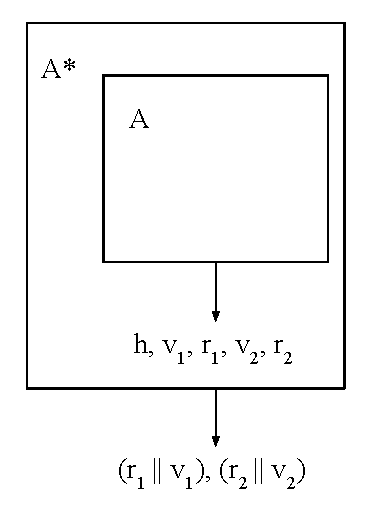
\includegraphics[width=0.35 \columnwidth,keepaspectratio]{figures/hash-commitment-reduction.pdf}
    \caption{The adversary $\mathcal{A}^*$ contains the code of $\mathcal{A}$ inside her. The outside
             adversary invokes the inside adversary to obtain the data that she later uses in her own
             response to her own challenger.}
    \label{fig.hash-commitment-reduction}
\end{figure}

\begin{theorem}[Commitment Security]
  The commitment scheme of Algorithm~\ref{alg.hash-commit} constructed using a \emph{secure
  hash function} $H$ is \emph{binding}.
\end{theorem}
\begin{proof}
  Consider any \emph{arbitrary}
  PPT adversary $\mathcal{A}$ that attempts to break the \emph{binding} property of the commitment scheme.
  We will prove that this adversary has only a negligible probability of success.
  We will construct a different adversary, $\mathcal{A}^*$, that attempts to break the \emph{collision resistance}
  property of $H$.

  The adversary $\mathcal{A}^*$ is depicted in \ref{alg.commit-security} and illustrated in
  Figure~\ref{fig.hash-commitment-reduction}. Let us observe some facts about these adversaries. First,
  the adversary $\mathcal{A}^*$ can make use of the adversary $\mathcal{A}$, because $\mathcal{A}^*$
  can simply have the code of $\mathcal{A}$ copy/pasted inside her own algorithm. Secondly,
  the adversary $\mathcal{A}^*$ is polynomial as long as $\mathcal{A}$ is polynomial, because
  $\mathcal{A}^*$ only executes a constant number of extra instructions in addition to invoking
  $\mathcal{A}$. Therefore, $\mathcal{A}^*$ is also a PPT algorithm. Lastly, these two adversaries
  will have different challengers: $\mathcal{A}$ is designed to succeed in the \emph{collision-game}
  challenger, while $\mathcal{A}^*$ is designed to succeed in the \emph{binding-game} challenger.
  One more thing to note is that we made this reduction without knowing anything about the
  nature of $\mathcal{A}$ beyond the fact that it is a PPT. Its code could be anything.

  Now for the probabilities of success, it is possible that $\mathcal{A}$ succeeds or fails.
  If $\mathcal{A}$ fails, we have no expectations of $\mathcal{A}^*$. But if $\mathcal{A}$ succeeds,
  then $\mathcal{A}^*$ always succeeds, too. The reason is the check performed by the \emph{binding-game}
  ensure that $\textsf{Verify}(h, v_1, r_1)$ and $\textsf{Verify}(h, v_2, r_2)$, but $v_1 \neq v_2$.
  But this means that $H(r_1 \conc v_1) = h$ and $H(r_2 \conc v_2) = h$, therefore
  $H(r_1 \conc v_1) = H(r_2 \conc v_2)$. But $r_1 \conc v_1 \neq r_2 \conc v_2$. To see this,
  note that $r_1$ and $r_2$ have the same length and could be equal, but $v_1$ and $v_2$ are different.
  Therefore, the check performed by the \emph{collision-game} will succeed.

  We conclude that, if $\mathcal{A}$ succeeds, then $\mathcal{A}^*$ succeeds, and s
  the probability of success of $\mathcal{A}^*$ against the \emph{collision-game}
  is at least as much as the probability of of success $\mathcal{A}$ against the \emph{binding-game}
  (in fact the two probabilities happen to be equal):

  \[
    \Pr[\textsf{collision-game}_{H,\mathcal{A}^*}(1^\kappa)] \geq
    \Pr[\textsf{binding-game}_{\textsf{Commit},\textsf{Check},\mathcal{A}}(1^\kappa)]
  \]

  From the assumption that $H$ is collision resistant, we know that

  \[
    \Pr[\textsf{collision-game}_{H,\mathcal{A}^*}(1^\kappa)] < \textsf{negl}\,.
  \]

  Therefore, applying the above inequality,
  $\Pr[\textsf{binding-game}_{\textsf{Commit},\textsf{Check},\mathcal{A}}(1^\kappa)] < \textsf{negl}$,
  too.
\end{proof}

This proof is a standard reduction proof that follows the outline we gave in Chapter~\ref{chapter.untrusty-world}.
Note how we skipped the $\kappa$ as a parameter to the \emph{negl} function, since it is clear
from context.

We proved that \emph{binding} follows from \emph{collision resistance}. It would seem that
\emph{hiding} must follow from \emph{preimage resistance}, but, even though this scheme is
hiding in practice, the proof will require a different model (see Problem~\ref{prob.preimage-no-hide}).

\section*{Problems}

\begin{enumerate}
  \item Consider a hash-based commitment scheme construction in which no salt is used.
        Prove that the scheme is correct. Use collision resistance to prove that the scheme is binding.
        Calculate the probability of success of a hiding adversary in the
        hiding game.\label{prob.commit-salt}
  \item Construct a correct commitment scheme which is hiding but not binding.
  \item Construct a correct commitment scheme which is binding but not hiding.
  \item Show that the hash-based commitment scheme constructed using a
        pathological secure hash function may not be hiding.
        (Hint: Start with a secure hash function $H$ and modify it
         to obtain a pathological secure hash function $H^*$.)\label{prob.preimage-no-hide}
\end{enumerate} % TODO: restore this file to build Ouroboros Proof-of-Stake later?

\section{Coins}\index{Transaction}
We are now ready to start creating money. Given our insight that money comes to be
through mutual social agreement---a social construct---we can create money simply by conjuring
it through software. As long as it is difficult to forge and everyone agrees
\emph{who has what}, it will become something that can take on value through social
agreement.

To solve the problem of knowing \emph{who has what}, we will employ an unusual strategy:
We will require that \emph{every node on the network knows who owns what}. There are privacy
and efficiency issues with this, and we will resolve both later.

Let us imagine how we can model the transfer of money between two parties. We need to represent
that Alice made a payment to Bob of some particular amount. We will represent this through a
\emph{transaction}. We will draw a transaction as a node (a circle) with an \emph{incoming edge}
and an \emph{outgoing edge}. The incoming edge is called the \emph{input}\index{Transaction input} and
illustrates \emph{who is paying}. The outgoing
edge is called the \emph{output}\index{Transaction output} and illustrates
\emph{who is getting paid}. We will draw the \emph{amount being transacted}
above the edge and \emph{the owner} below the respective edge. A transaction of $1$ unit
between Alice and Bob is illustrated in Figure~\ref{fig.utxo-transaction}. This may seem like
an unusual way to illustrate things, but it will soon become clear why we are adopting it.

\begin{figure}[h]
    \centering
    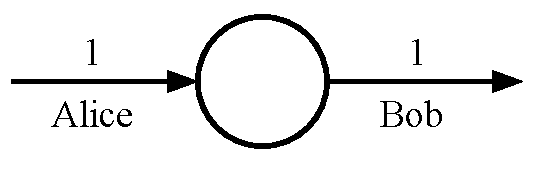
\includegraphics[width=0.35 \columnwidth,keepaspectratio]{figures/utxo-transaction.pdf}
    \caption{A transaction paying $1$ unit of money from \emph{Alice} to \emph{Bob}.}
    \label{fig.utxo-transaction}
\end{figure}

For Alice to spend this money and give it to Bob, she must have been given this money previously.
We will illustrate this by the output of one transaction connecting to the input of another,
as illustrated in Figure~\ref{fig.utxo-transaction-chain}.

\begin{figure}[h]
    \centering
    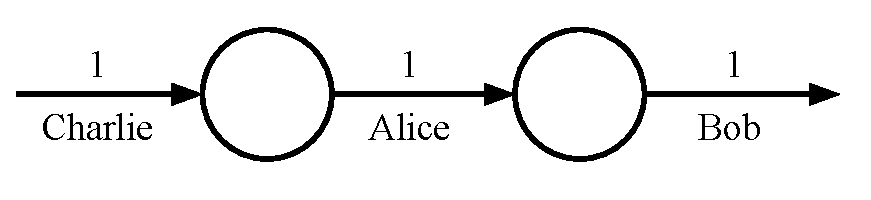
\includegraphics[width=0.55 \columnwidth,keepaspectratio]{figures/utxo-transaction-chain.pdf}
    \caption{\emph{Alice} pays $1$ unit of money to \emph{Bob}. She received this money from \emph{Charlie}.}
    \label{fig.utxo-transaction-chain}
\end{figure}

Money changing hands in this manner is referred to as a \emph{coin}\index{Coin}. A coin has a current owner,
denoted in the final outgoing output edge which is not connected to another transaction as input.
It has a history of previous owners. The outgoing output
edge of a transaction that is not connected to another transaction is an output \emph{available for spending}.
It is a \emph{dangling output} and
it is known as an \emph{Unspent Transaction Output} (UTXO)\index{UTXO}.

As we discussed in the signatures section, we will use public keys for identities. Our transactions
will not contain a payment from ``Alice'' to ``Bob'', but from some public key (whose respective secret key
is held by Alice) to some other public key (whose respective secret key is held by Bob). This is
illustrated in Figure~\ref{fig.utxo-transaction-keys}. However, for convenience, we will write out
\emph{Alice} and \emph{Bob} in place of their public keys, understanding that the payments are
made to public keys and not legal identities. An appropriately encoded public key to which a payment can be made is
also known as an \emph{address}\index{Address}. An address can be exchanged between counterparties
even before any transaction takes place.

\begin{figure}[h]
    \centering
    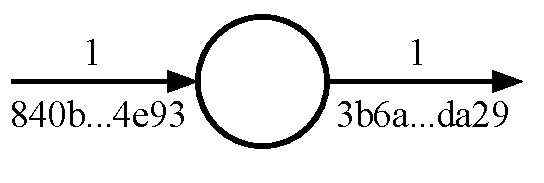
\includegraphics[width=0.35 \columnwidth,keepaspectratio]{figures/utxo-transaction-keys.pdf}
    \caption{A transaction pays from one public key to another. It does not contain real names
             or other identifying information.}
    \label{fig.utxo-transaction-keys}
\end{figure}

\section{Multiple Outputs}

It may be useful to pay for multiple things with a single transaction. If Alice receives
her salary through one transaction, she may want to spend it on both her rent as well
as on a book. A transaction can have multiple outputs. Each of the outputs may have a,
potentially different, recipient public key and a, potentially different, amount.
An example is illustrated in
Figure~\ref{fig.utxo-multiple-outputs}. Each of the outputs can be spent independently.
For example, Alice's landlord can spend his money while the bookstore doesn't. This
transaction consumes one input and produces two outputs.

\begin{figure}[h]
    \centering
    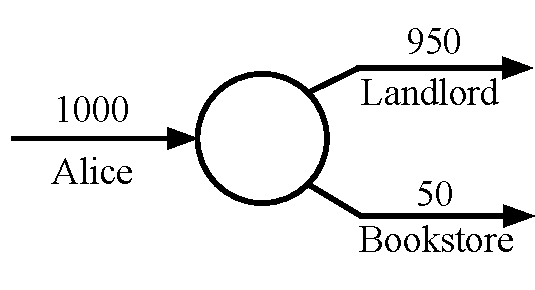
\includegraphics[width=0.35 \columnwidth,keepaspectratio]{figures/utxo-multiple-outputs.pdf}
    \caption{Alice uses her salary, the incoming edge, in a single transaction to pay for
             both her rent and a book in two different outgoing edges.}
    \label{fig.utxo-multiple-outputs}
\end{figure}

An outgoing edge can either be spent (if it is connected to another transaction) or
unspent (if it is not connected to another transaction). It cannot be partially spent.
A UTXO can only be spent in its \emph{entirety} by being connected as input to a new
transaction. If Alice wants to use \emph{part} of her salary to buy a book, and keep
the rest of her salary for later spending, she must still spend her salary output
in its entirety and use it as a transaction input. She creates \emph{two} outputs
in this transaction: One paying the bookstore, and the other paying back to herself.
The second output is the new UTXO that she can use to spend her remaining salary
at a later time. This is known as a \emph{change output}\index{Change} and is
illustrated in Figure~\ref{fig.utxo-change}.

\begin{figure}[h]
    \centering
    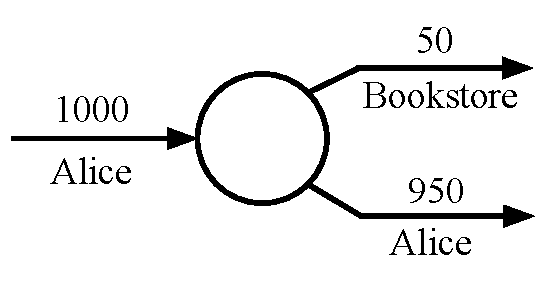
\includegraphics[width=0.35 \columnwidth,keepaspectratio]{figures/utxo-change.pdf}
    \caption{Alice uses her salary, the incoming edge, in a single transaction to pay for
             a book (top output edge). She uses the rest of her money to pay the
             \emph{change} back to herself (bottom output edge).}
    \label{fig.utxo-change}
\end{figure}

Coins are often spent in a series of transactions like that. Alice uses her salary
to pay for a series of things. She first pays for a book, then gives herself the change
of that transaction. In a next transaction, she pays for an apple, and then gives herself
the change of that. She then pays for a coffee, and gives herself the change for that.
This process is illustrated in Figure~\ref{fig.utxo-change-chain}. This graph has four
UTXOs: Alice's remaining salary of $944$ units, the payment for the book store of $50$
units, the payment to the fruit market for $1$ unit, and the payment to the coffee shop
for $5$ units. The left-most edge, Alice's original salary of $1000$ is not a UTXO, since
it is spent. Even though there are four UTXOs, only three transactions are depicted in this
graph.

\begin{figure}[h]
    \centering
    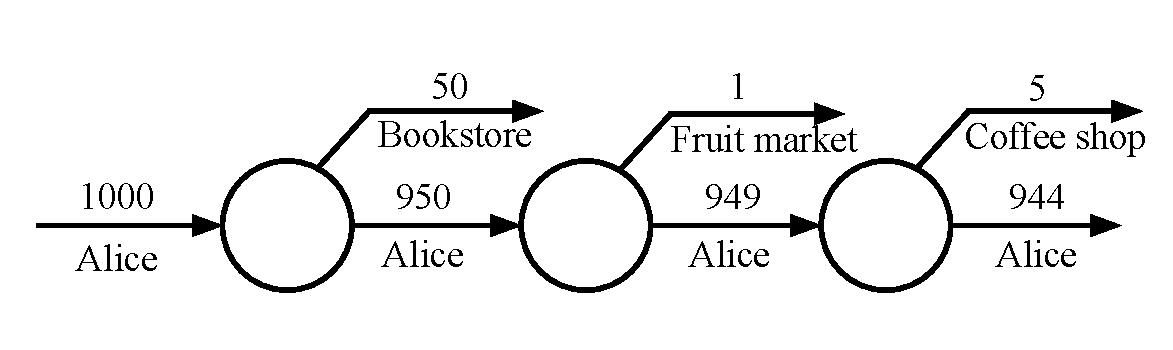
\includegraphics[width=0.75 \columnwidth,keepaspectratio]{figures/utxo-change-chain.pdf}
    \caption{Alice uses her salary, the left-most edge, in a series of transactions,
             always giving change back to herself. The bottom-right edge is her remaining salary.}
    \label{fig.utxo-change-chain}
\end{figure}

\section{Multiple Inputs}

It is also possible to \emph{combine} multiple inputs into a single transaction to make
a larger payment. For example, Alice can use two of her salaries, each of which resides
in a different transaction output, to make a down payment for the house she is buying.
This is illustrated in Figure~\ref{fig.utxo-multiple-inputs}. This transaction consumes
two outputs and produces one new output.

\begin{figure}[h]
    \centering
    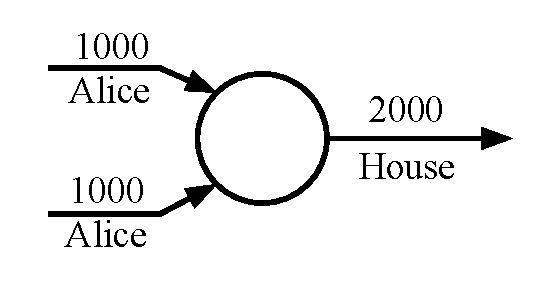
\includegraphics[width=0.35 \columnwidth,keepaspectratio]{figures/utxo-multiple-inputs.pdf}
    \caption{Alice combines two of her salaries (left, incoming edges) to pay for her
             house (right, outgoing edge).}
    \label{fig.utxo-multiple-inputs}
\end{figure}

Typically, a transaction will have one or more inputs and exactly two outputs. Alice will use
one or more payments she has received (including previous change) to pay for something she is
purchasing, and give herself the change remaining from the purchase.

\section{The Conservation Law}

Money needs to be scarce. When money is transacted, new money must not be created out of nothing.
The input amounts to a transaction must
match the output amounts of the same transaction. This is known as the \emph{conservation law}.
Let us denote by $\tx$ a transaction, by $\tx\textsf{.ins}$ its array of inputs,
and by $\tx\textsf{.outs}$ its array of outputs. For each input \emph{in} in
$\tx\textsf{.ins}$, let us denote by $\textsf{in.v}$ the amount in the particular
input, and similarly for \emph{out}. We can write the conservation law in an equation.

\begin{definition}[Conservation Law]
  Given a transaction $\tx$, we say that it obeys the \emph{Conservation Law} if

  \[
    \sum_{\textsf{in} \in \tx\textsf{.ins}} \textsf{in.v} = \sum_{\textsf{out} \in \tx\textsf{.outs}} \textsf{out.v}
  \]
\end{definition}

Most transactions will obey this law. However, money must come from \emph{somewhere},
and so there must be some initial transactions that do not obey this law. These are known as
\emph{coinbase} transactions. Even though they have valued outputs, they have no inputs. They
are the only ones that do not respect the Conservation Law.
Coinbase transactions follow very particular rules and they must be designated and limited,
in order to have scarcity.
We will explore the exact rules
in more detail when we speak about macroeconomics in Chapter~\ref{chapter:chain}.
Even though there can be transactions with no inputs (the coinbase transactions), every
transaction must have at least one output.

\section{Outpoints}

Each transaction is given an \emph{identifier} known as the \emph{$\txid$}~\index{txid}. This is
obtained by hashing the transaction data (including all of its inputs and outputs).

Since an input of a transaction is always spending a previous output, the input can just be a
reference to a previous output. To reference an output, we need to specify the transaction it
belongs to, using its $\txid$, as well as the \emph{index} of the output (whether it is the first
output of the transaction, or the second output of the transaction, and so on). The pair
$(\txid, \idx)$ is used in place of an input and is sufficient to uniquely specify a previous
output. The value $\idx$ is simply a number $0, 1, 2, \ldots$.
This pair is known as an \emph{outpoint}\index{Outpoint}. An outpoint example is illustrated
in Figure~\ref{fig.utxo-outpoint}. We will illustrate the outpoint pair on top of an
incoming edge to a transaction, although this will typically be implicit.

\begin{figure}[h]
    \centering
    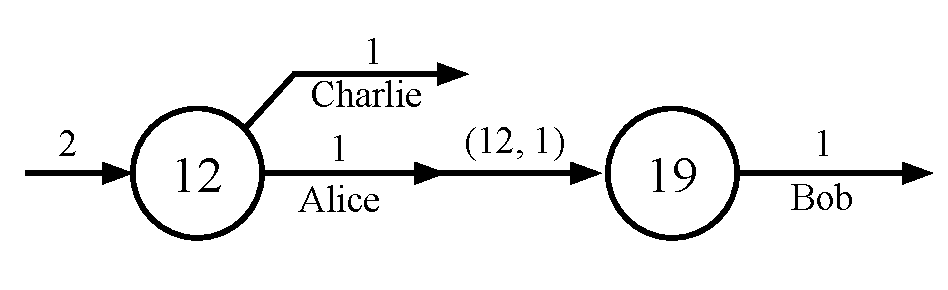
\includegraphics[width=0.65 \columnwidth,keepaspectratio]{figures/utxo-outpoint.pdf}
    \caption{The transaction number $19$ has a single input that spends the output number $1$ (to Alice)
             of transaction number $12$.
             The output number $0$ of transaction number $12$ (to Charlie) is still unspent.
             Here, we have highlighted the outpoint pair $(12, 1)$ that connects the input
             of transaction $19$ with the specific output of transaction $12$.}
    \label{fig.utxo-outpoint}
\end{figure}

\section{The UTXO Set}

The whole history of payments in our system forms a \emph{transaction graph}\index{Transaction graph}.
This is a Directed Acyclic Graph (DAG). It cannot contain cycles because transactions must be
strictly orderable in the way that they spend: the input of a next transaction refers to
outputs of previous transactions through outpoints that contain their hashes in the form of $\txid$s.
An example transaction graph is illustrated in Figure~\ref{fig.utxo-tx-graph}. In this diagram,
we are not showing the edge owners or amounts for conciseness. As new payments are made in the system,
new transactions are added to the graph, but existing transactions are not modified, and previously
added transactions are not removed. This is an append-only graph.

Some transactions in the graph have outputs that have all been spent, and we will never need to care
about them again. Some transactions have dangling outputs, and so their outputs are available for
spending. The money that is available for spending in the system is in the UTXOs. The set of all UTXOs
forms the \emph{UTXO set}\index{UTXO set}.

Transactions in the transaction graph can be ordered in a sequence of transactions. We can do this
by ordering the graph in topological order. We start with an empty sequence of transactions and we
place the transactions from the graph into the sequence one by one, ensuring each transaction appears
only once. The strategy we use to place transactions in the sequence is that we always choose a transaction
whose inputs point to transactions that have all already
been placed in the sequence. Since coinbase transactions have no inputs, they can always be placed in the sequence.
We continue
in this manner until all transactions have been placed into our sequence. There may be multiple
ways to order transactions in this manner, but there will always be one way to do it. All of the ways
are \emph{consistent}: each transaction
that spends from another transaction is placed in the sequence \emph{after} the transaction that it spends
from. This sequence of transactions, ordered in this consistent manner, is known as a
\emph{transaction ledger}\index{Ledger}. In Figure~\ref{fig.utxo-tx-graph}, transactions are labelled
in one possible consistent order. As new transactions are added to our graph, they can also be appended
to the transaction ledger while maintaining consistency.

\begin{figure}[h]
    \centering
    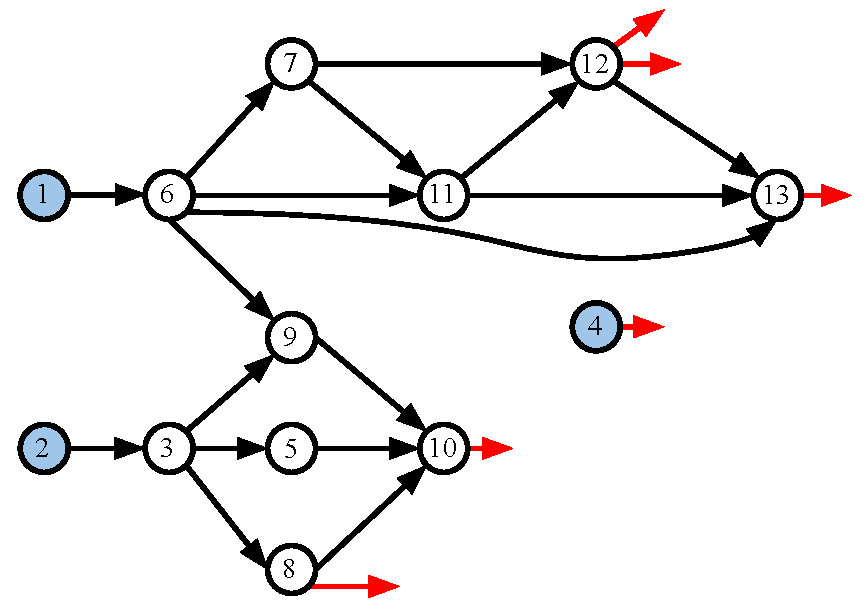
\includegraphics[width=0.65 \columnwidth,keepaspectratio]{figures/utxo-tx-graph.pdf}
    \caption{A transaction graph with $3$ coinbase and $10$ non-coinbase transactions.
             Coinbase transactions are shaded blue.
             There are $23$ outputs, of which $6$ belong to the UTXO set.
             The UTXO set is shaded red. Transaction number $8$ contains both
             a spent and an unspent transaction output.}
    \label{fig.utxo-tx-graph}
\end{figure}

Each node in our network stores the \emph{whole} transaction graph. When a party wishes to make
a payment, they create a new tranasction and broadcast it to the network. This transaction is
received by the other peers, who add it to their local transaction graph. Now everyone
knows \emph{who owns what} by looking at their local UTXO set. The sum of all the values
in the UTXO set is equal to the total amount of money in the system.

In particular, if I, as an honest node, want to know \emph{how much money I have}, I look
at my local UTXO set and collect all those UTXOs who are marked with a public key whose
respective private key I am in possession of. Summing all of their values gives me my
current holdings.

\section{Transaction Signatures}

For a transaction to be valid, its inputs must point to outputs whose spending has
been authorized by their rightful owner. This can be done by \emph{signing} the new transaction
data using the secret key that corresponds to the public key annotated on the previous output
being spent.
Let us look at the transaction that Alice creates in Figure~\ref{fig.utxo-sig}. This
new transaction, transaction $19$, is spending from an output that belongs to Alice.
The output being spent is the output with index $0$ of transaction $7$.
The new transaction is paying Bob $1$ unit and Charlie $2$ units, for a total of
$3$ units.

\begin{figure}[h]
  \centering
  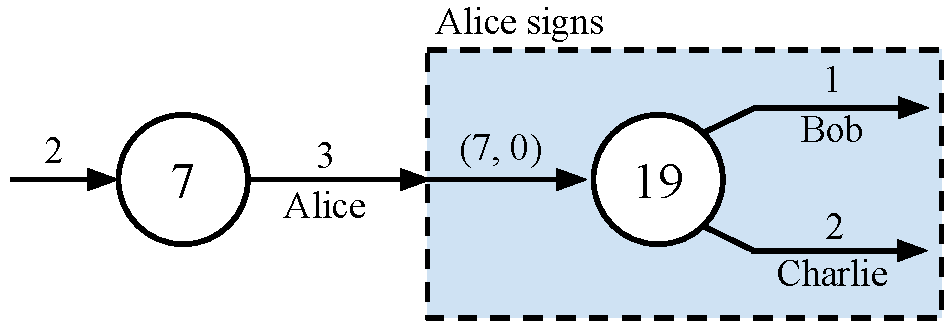
\includegraphics[width=0.65 \columnwidth,keepaspectratio]{figures/utxo-sig.pdf}
  \caption{Alice creates a new transaction, transaction $19$, by which she pays Bob
           $1$ unit
           and Charlie $2$ units.
           The transaction data include Bob's public key, Charlie's public key,
           the outgoing amounts $1$ and $2$, and the outpoint $(7, 0)$.
           These must all be signed by Alice's secret key.}
  \label{fig.utxo-sig}
\end{figure}

Alice must authorize this spending by signing using her secret key.
The data that she signs are the contents of the new transaction:
The owners and amounts in the outputs, and the outpoint of the input.
It is not necessary to include the value of the input here, as the outpoint
uniquely identifies it. It is imperative that Alice includes the public key
of Bob in her signature when she creates this transaction. Otherwise, a malicious
party, Eve, on the network could swap out Bob's public key with her own. If a secure
signature scheme is used, any such forgery will be impossible due to existential
unforgeability. The same applies in case Bob attempts to alter the amounts allocated
to him and Charlie: Alice's signature will be invalidated, and the transaction will
no longer look valid to any observers. Alice's signature on the transaction is packed
together with the transaction and accompanies it whenever it is broadcast on the network.

\begin{figure}[h]
    \centering
    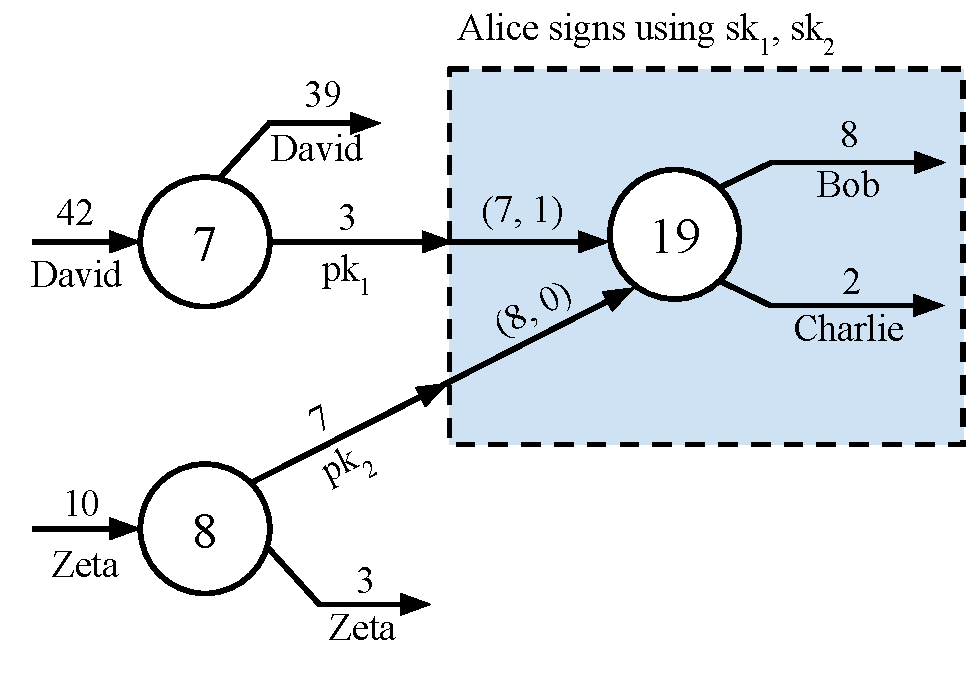
\includegraphics[width=0.65 \columnwidth,keepaspectratio]{figures/utxo-sig-multi.pdf}
    \caption{Alice creates a new transaction, transaction $19$, by which she pays Bob
             $8$ units
             and Charlie $2$ units.
             The transaction data include Bob's public key, Charlie's public key,
             the outgoing amounts $1$ and $2$, and two outpoints, $(7, 1)$ and $(8, 0)$.
             All of these data must be signed twice: Once using Alice's $sk_1$ secret key,
             and once using Alice's $sk_2$ secret key, giving two different signatures
             $\sigma_1$ and $\sigma_2$ on the same data.}
    \label{fig.utxo-sig-multi}
\end{figure}

If Alice wishes to create a transaction with multiple inputs she controls, she must
provide a signature corresponding to each of the inputs. Consider the example illustrated
in Figure~\ref{fig.utxo-sig-multi}. Here, Alice wishes to spend two outputs that she
owns. The first output has been paid to Alice's public key $pk_1$. The second output
has been paid to Alice's public key $pk_2$. Alice controls the respective secret keys
$sk_1$ and $sk_2$. Alice creates a new transaction, transaction $19$, containing the
desired inputs and outputs. In the inputs, she places two outpoints pointing to the
two outputs she wishes to spend. The new transaction data, including the inputs and outputs,
must all be signed twice: First, using Alice's $sk_1$ (and verifiable using $pk_1$),
and secondly using Alice's $sk_2$ (and verifiable using $pk_2$). This will yield two
different signatures $\sigma_1$ (created using $sk_1$) and $\sigma_2$ (created using
$sk_2$). Both of these signatures verify on the \emph{same} data, but using different
public keys. A signature for the outpoint connected to each of the transaction's inputs
must accompany the transaction whenever it is broadcast. A transaction is accompanied
by as many signatures as it has inputs.

\section{Transaction Creation}

When the honest node Alice wishes to create a new transaction, she performs the following steps:

\begin{enumerate}
  \item She requests the public key of the recipient through some off-chain means (e.g., via e-mail or a QR code).
  \item She picks the UTXO outputs she wishes to spend from.
  \item She creates a new transaction with the output \emph{public keys} and \emph{amounts} she wishes to pay to.
  \item She creates transaction inputs where she places outpoints pointing to the UTXOs she wishes to spend from.
  \item She collects all the above transaction data into a message.
  \item For each of the outpoints, she uses her respective private key to sign the message.
  \item She broadcasts the transaction and its signatures to the network.
\end{enumerate}

\section{Transaction Format}

So far, we have treated a transaction as an abstract object. It is time to make this concrete. A transaction
consists of its \emph{inputs} and \emph{outputs}:

\begin{enumerate}
  \item Its list of \emph{inputs}. Each element in this list is an outpoint, a pair in the form $(\txid, \idx)$.
  \item Its list of \emph{outputs}. Each element in this list is a pair containing a public key
        (the owner of the output) and an integer amount.
\end{enumerate}

An example transaction object looks like this:

\begin{verbatim}
  {
    inputs: [
      {
        outpoint: (
          "cc6a88afaca94fec238258e3665d64cd
           de592e3ea13f151eca37d5e6589cd169",
          0
        )
      },
      {
        outpoint: (
          "3a648c42b90af46b9bba7ae723451002
           aa53baba187020051e0c32112bf458a0",
          3
        )
      }
    ],
    outputs: [
      {
        pk: "36dec8c46741efdab93a77f8fc75acec
             6e290b1ce0f280e04753db5c864a6469",
        amount: 5012900000000
      },
      {
        pk: "f71c1e7478459d90764d59dd9cb0ea9f
             62406d2c1412dea7c6de0c0355183066",
        amount: 3170000000000
      },
      {
        pk: "d9169b9601f3121f316f44e4d1bd0ecc
             d6d07df4d152fdcbf59a210e7c77e467"
        amount: 135000000000
      }
    ]
  }
\end{verbatim}

The amounts are given as integers. These are given in
the smallest denomination possible that we want to allow our cryptocurrency to take.
For example, Bitcoin uses the \emph{satoshi} unit, equal to
$10^{-8}$ bitcoin, whereas Ethereum uses the \emph{wei}, equal to
$10^{-18}$ ether. The coins cannot be further divided beyond integer amounts.
This avoids floating point errors.

The transaction example above is an \emph{unsigned} transaction, and cannot be
broadcast to the network as-is. Signatures must be included with each outpoint
to authenticate the respective input. A \emph{signed} transaction looks something
like this:

\begin{Verbatim}
  {
    inputs: [
      {
        outpoint: (
          "cc6a88afaca94fec238258e3665d64cd
           de592e3ea13f151eca37d5e6589cd169",
          0
        ),
        sig:
          "680b733e57690024d18025603f6df238
           b6f181c2de76b96961a90c1f0fc0d1e2
           42795ddd48f06e6ac2760579459b6b98
           ef77d91c4278dd0a9feaac91a57eae08"
      },
      {
        outpoint: (
          "3a648c42b90af46b9bba7ae723451002
           aa53baba187020051e0c32112bf458a0",
          3
        ),
        sig:
          "13f1eb894921c7535ac51aac874187ac
           993b0dcf7b3b439b15cf408dbf66db2b
           7739605ef9ab0bc79be7957a9e15ef0b
           e0dd92524c8881cc3fd3742c621e8c0b"
      }
    ],
    outputs: [
      {
        pk: "36dec8c46741efdab93a77f8fc75acec
             6e290b1ce0f280e04753db5c864a6469",
        amount: 5012900000000
      },
      {
        pk: "f71c1e7478459d90764d59dd9cb0ea9f
             62406d2c1412dea7c6de0c0355183066",
        amount: 3170000000000
      },
      {
        pk: "d9169b9601f3121f316f44e4d1bd0ecc
             d6d07df4d152fdcbf59a210e7c77e467",
        amount: 135000000000
      }
    ]
  }
\end{Verbatim}

Naturally, the particularities of how transactions are encoded differ from blockchain
to blockchain in practice. For example, Bitcoin uses the \texttt{secp256k1} signature
scheme to produce the public keys to receive payments and
\texttt{sha256} as the hash by which $\txid$ is calculated.
In contrast, Ethereum uses the \texttt{keccak} hash to calculate $\txid$,
and Cosmos Hub uses the \texttt{ed25519} signature scheme to generate public keys.
The encoding of addresses also differs from cryptocurrency to cryptocurrency.
For example, Bitcoin encodes addresses by taking the public key,
hashing it with two different hashes (\texttt{ripemd} and \texttt{sha256}),
and then applying the \texttt{base58}
encoding function which adds some checksums to avoid mistypes.
These details are implementation details and are immaterial to the foundational
functionality of the system.

\section{Transaction Validation}

In order to verify an incoming transaction from the network, each node must maintain the current transaction
graph and in particular the \emph{current UTXO set}.
When a node sees a new transaction arriving from
the network, it checks the new transaction's inputs to see if they belong to its current UTXO set.
If the transaction is valid, the node adds the new transaction to its transaction graph.
It also removes the new transaction's inputs
from its \emph{current UTXO set}, and adds the new transaction's outputs to its \emph{current UTXO set}.
This is how the transaction graph and the current UTXO set of each node evolve.

When a new transaction arrives at the door of a receiver for the first time, he must check that it is
a valid transaction. This process is called \emph{transaction verification}. It involves checking that
this transaction is rightfully spending the money that it is claiming. If a transaction is deemed \emph{valid},
then it is gossiped to the rest of the network. If a transaction is deemed \emph{invalid}, then it is
rejected, and it is not gossiped to the network. This protects from spammy transactions occupying the
network. The checks performed when verifying a transaction include checking the Conservation Law
and checking the signatures on the new transaction.

To perform these checks, he must follow the outpoints to find out the corresponding
public keys and amounts. When the honest party  Bob wishes to verify a transaction $\tx$ received from
the network, he performs the following steps:

\begin{enumerate}
  \item For each transaction input, he resolves the respective outpoint.
  \begin{enumerate}
    \item He checks that this outpoint is in his current UTXO set. \label{enum.tx-double-spend}
    \item He retrieves the public key and amount of this outpoint.
    \item He checks that a signature on the new transaction data verifies using the public key of the outpoint.
  \end{enumerate}
  \item He checks that the Conservation Law holds (or that this is a valid coinbase transaction).
  \item He removes the outpoints from his current UTXO set.
  \item He adds the new outputs to his current UTXO set.
\end{enumerate}

Let us discuss the step~\ref{enum.tx-double-spend} above.
This is a necessary condition to ensure that the money really \emph{does} belong to its rightful owner and
has not been previously spent.
Consider what it would mean if this step failed.
The verifier here is seeing a \emph{new} transaction, a transaction he has never seen before.
Yet, this transaction is spending from an output that is \emph{not} in his UTXO set.

It's possible that \emph{this outpoint was never added to the UTXO set in the first place}.
This can occur for two different reasons.
The first reason is malicious. The adversary is creating a transaction spending from
a non-existing outpoint. This transaction must be rejected.
The second reason is benign, and it is a \emph{race condition}.
If Alice pays Charlie in one transaction $\tx_1$ and then Charlie pays David in another
transaction $\tx_2$, which spends from $\tx_1$, then $\tx_1$ and $\tx_2$ will be broadcast
in this order. However, the verifier may receive them on the network
in a different order than they were sent. He can see $\tx_2$ first, and $\tx_1$ only later.
If a verifier sees $\tx_2$ first, then
he cannot verify this transaction before he has seen $\tx_1$. After all, he doesn't have
the necessary public key to verify the respective signature, and he doesn't have the
necessary amounts to verify the Conservation Law.
He must necessarily \emph{reject}
$\tx_2$. It is not
the responsibility of the verifier to hold onto $\tx_2$ until $\tx_1$ is received,
because he cannot know if such a $\tx_1$ exists in the first place. For all it knows,
an adversary could be attempting to spend a non-existent outpoint.

Alternatively, it's also possible that \emph{this outpoint was added to the UTXO set, but was later
removed from the UTXO set}. This means that there exists a different transaction
which spends from the \emph{same} output. This is called a \emph{double spend},
and it must be rejected. Double spends are necessarily adversarially created.
Honest parties do not produce double spending transactions.

\begin{definition}[Double Spend]
  In the UTXO model, a transaction $\tx$ is a \emph{double spend} or a
  \emph{conflicting transaction} with another transaction $\tx' \neq \tx$,
  if $\tx$ and $\tx'$ both have some outpoint in their inputs that is the
  same, i.e.,

  \[
    \exists i, j \in \mathbb{N}: \tx\textsf{.ins}[i]\textsf{.outpoint} = \tx'\textsf{.ins}[j]\textsf{.outpoint}
  \]
\end{definition}

Transactions broadcast from different parts of the network may arrive in a different order in other
parts of the network.
As different nodes on the network see different transactions
at different times, each node may have a different opinion on what their current UTXO set is.
This can lead to race conditions, which we tackle in the next chapter.

\section*{Problems}

TBD

\section*{Further Reading}

The UTXO model was first put forth in the context of Bitcoin by Satoshi Nakamoto. Satoshi
introduced blockchains, and his paper, \emph{Bitcoin: A Peer-to-Peer Electronic Cash System}~\cite{bitcoin} is
the seminal paper that spoke about them for the first time. Consider it mandatory reading.
It is an easy and short paper that includes details about the UTXO model that we explored
in this chapter, but also blocks, chains, and SPV proofs that we will explore in the next chapters.
The denomination \emph{satoshi} in Bitcoin is named after Satoshi Nakamoto.
Satoshi was a pseudonym of an alleged Japanese man
who created both the Bitcoin paper and the first Bitcoin implementation in C++ during the years
2008-2009. After two short years of participation in the community, he disappeared mysteriously, never
to be heard from again. His identity remains a mystery.

For many more details on transaction format particularities in the specific implementation of the UTXO
model in Bitcoin, refer to the Bitcoin Developer Guide~\cite{bitcoin-dev-guide}.
The books Mastering Bitcoin~\cite{mastering-bitcoin} and Mastering Ethereum~\cite{mastering-ethereum}
go into a lot of detail about the particularities of transaction, key, and address formats
for Bitcoin and Ethereum respectively.

% TODO: Make sure these are covered
% \item What money do I own? Calculating balances / Wallets as a collection of keys
% \item Reading: Chapter 5 introduction and section 5.1 from Modern Cryptography (2nd ed.)
% \item Reading: Chapter 12 introduction (skip comparison to MACs and relation to encryption) and sections 12.1, 12.2, 12.3 from Modern Cryptography (2nd ed.)
